\section{Sorting recap}
\label{sec:sorting_recap}

\begin{frame}
	\frametitle{To summarise}
	\framesubtitle{XKCD Ineffective Sorts: \url{https://xkcd.com/1185/}}
	\begin{center}
		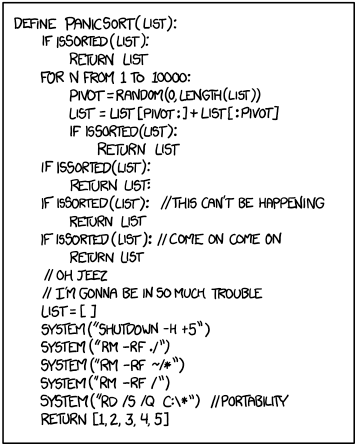
\includegraphics[width=0.4\textwidth]{figures/panicsort.png}\\
	\end{center}
\end{frame}

\begin{frame}
	\frametitle{Summary table}
	\begin{tabular}{r | c | c | c}
		\small
		Sorting method & Time & Main advantage & Main disadvantage \\
		\midrule
		Bubble Sort & $O(n^2)$ & Easy for humans! &  Very very very very slow \\
		Insertion Sort & $O(n^2)$ & Good for small lists &  Still quadratic time \\
		Selection Sort & $O(n^2)$ & Good for small lists &  Still quadratic time \\
		Merge Sort & $O(n \log n)$ & Faster than quadratic! &  Bad on `almost sorted lists' \\
		Quick Sort & $O(n \log n)$\footnote{in expectation} & Faster than merge sort &  Still worst-case quadratic\dots \\
	\end{tabular}
	\begin{itemize}
		\item We can mix Bucket Sort in with all this, by applying it first and then applying it (or one of the others) on
			the different buckets.
		\item Sorting algorithms can be in-place or not and stable or not.
	\end{itemize}
\end{frame}

